\iflanguage{ngerman}
{\chapter{Ergebnisse}}
{\chapter{Evaluation}}

\label{sec:evaluation}


% Linerenderer conponent also produces large overhead due to the amount of gameobjects it creates
% Need to test when Dataset gets to large for my PC to handle
% Also add expert feedback
% objektive comparison of presented methods 
% Forced based approach spacing force F_s needs imporvment as algorithm is slow (O(n^2))
% informal quality analysis? 
% waht could be done to improve the visuallisation of dynamic datasetss?
% Are exploded Views really viable for that?

\section{Qualitative Analysis}
In order to evaluate the developed methods, first a qualitative analysis is performed, in which the individual methods are discussed and evaluated with the results of the expert evaluation, followed by a quantitative analysis, which is done by conducting a performance test.
The expert feedback was recorded in a meeting with two external scientists of the TU Dresden and developers of the Morpheus program. For this, the developed methods were first presented, then both had time to try out the methods themselves. A first generation HTC Vive was used and notes on feedback were taken during testing, then questions were asked about effectiveness, usability and areas for improvement, the specific questions can be found in the appendix(\ref{ExpertQuestions}). Both experts stated that they had little to no experience with virtual reality headsets.
Overall, there was very positive feedback on the methods presented and the possibilities they offer for exploring the data sets.
They also stated that the various methods are all useful in different ways and that no single method is best for every application.
Positively, it was pointed out that both the occlusion that occurs can be avoided with the methods and the context of the cells is preserved, thus achieving the goal of the work.
It was also noted that context preservation is not always desirable and that it can be useful to break it up in order to better extract other desired information.
The ability to extract and view individual cells was also found to be very useful and intuitive.
Furthermore, a variety of extension possibilities and suggestions for improvement of the methods were made.
According to how they are used, the various techniques are to be classified as follows.


\subsection{Point explosion}
The point explosion is the easiest method to understand and helps the viewer to get an understanding of the composition of the object, especially for the initial observation.
Here it is easy to orientate and select individual parts of the data set.
The ease of use with only one control point is also helpful here, as well as the steadier expansion compared to the other methods presented.
With this method, the context of a single cell is hard to see, as cells that are close to each other can be far apart in the exploded view. However, according to the experts, this is not decisive, since a good mental reconstruction of the cell complex is still possible. Also, this exploded view leads to a well presentable visualization, which is easily understandable even for uninformed people, since the object structure and shape remain similar.
However, the implemented length factor does not have the desired effect here and is more of a hindrance, since it breaks up the original cell structure, which is important for the mental reconstruction.
Here, an effect radius as described by Sonnet et al. might be more useful.
It could also be advantageous to be able to set the explosion point, from which the explosion originates, directly on individual parts, so that these remain at their original position.
This is currently possible if the effect point is set to the reference point of the part, but is difficult in practice because the necessary precision is not available with the controllers.
The point explosion is therefore particularly suitable for orienting oneself in the data set and quickly gaining an understanding of the rough object structure and the object interior.

\subsection{Line explosion}
The line explosion has proven to be the most effective method for analytical observation. Due to the possibility of exploding the object only partially, when the control point is placed inside the cell complex, the mental reconstruction is facilitated and the context is better preserved.
Nevertheless, it is possible to inspect the interior of the cell complex and the individual cell interactions. If the dataset is scaled to a small size, the head-mounted method can be used to easily view the interior of the cell from each side. As all parts that are in front of the control point are dynamically pushed away. This allows for an easy intuitive inspection of the cell and its composition. Although the operation of the control points in the original implementation is a bit cumbersome, the expansion of the parts is still easy to understand. The interaction is improved with the head-mounted method, as there is only one control point that needs to be placed. One improvement that has been suggested is easier switching between the head-mounted method and normal line explosion using two control points. 
This is currently implemented as a toggle using a UI panel and could be improved if this is set to a button on the controller to be able to quickly switch between the view-dependent and view-independent version. Adjusting the three factors F1, F2, and F3 can effectively be used to either better represent the composition or allow an unobstructed view of the cell interior. These options also allow flexible customization of the exploded view depending on whether context preservation or free representation is desired. The experts found the method to be intuitive, reactive and interactive, but also had a number of suggestions for improvement. For example, the naming of parameters and methods was considered to be not very meaningful. Here it could help to make the naming less implementation-oriented and to promote a better mental model of the user. In the HCI, this is described as gulf of evaluation and describes the discrepancy between what the system displays and what the user expects. So the current naming is too system-centered and could be improved by considering the factors $F_1$ to $F_3$ as parameters of a cone. This deviates slightly from the implementation, but creates a more representative metaphor for how the parameters work.
Furthermore, it was suggested that the method be could called conic explosion instead of line explosion to reinforce this mental model. This could also change the current interaction, in that the user no longer adjusts the two control points and then changes the parameters, but can move a cone-shaped object that can be scaled and changed by gestures. This could then be pushed into the model and thus determines the expansion of the parts. The parameters would thus be mapped more intuitively as a three-dimensional object, which is much easier for the user to understand. Nevertheless, this method, especially with the extension to the view-dependent view, has proven to be the best method for analytical examination. It can be used best for exploring the object structure and still get a good understanding of the composition.

\subsection{Force-based explosion}
The force-based method uses a different approach to create the exploded view than the other methods. The advantage of this is the dynamic nature of the explosion created. Any number of target parts can be selected here to define the explosion. Because the target parts remain in their original positions, it is possible to select a subset of the dataset and view it while pushing away all other parts. So it is possible to view groups of cells over time without completely hiding the others. If the viewing force is increased, all parts that are not target parts are pushed away from the viewing direction. This allows an unobstructed view of the selected parts and has a similar effect as if these parts were deactivated. However, since this is not the case and the parts are merely pushed away, the object structure is preserved better than if the parts were only hidden. Because the explosion emanates from all selected parts, the view is particularly useful for viewing cells that make a large spatial change, as all parts are dynamically moved away from it. A problem, which occurs due to the implementation, is the sluggishness, with which the cells move. This is partly due to the drag value of the Unity Physics objects. This value introduces friction into the calculation and reduces jittering of the parts when they bounce beyond their target position. A downside of this, however, is that the parts become less responsive. This can be partially counteracted by increasing the strength of all forces. However, finding suitable values that both generate a good explosion view and allow parts to jump quickly to their final position without moving beyond their target position remains a difficult task. Furthermore, the implementation of the spacing force needs improvement, as here every part is tested against each other resulting in an $O(n^2)$ complexity of the algorithm. This exponential complexity quickly leads to performance problems as the number of parts increases. This is where using a spatial hashgrid, into which each part is inserted and each part is checked only against the parts in adjacent grid segments, might help. The method is therefore most useful when a group of cells and their development over a period of time is to be examined more closely. It serves as a middle ground between the simpler point explosion and the more complex line explosion.

The discussion with the experts also led to further suggestions for improvement, which could be explored. For example, it was suggested to refrain from the implemented egocentric view and the current locomotion system and to create an observer view, in which the user does not move in space, but instead the dataset is transformed. This could make orientation easier as well as navigating the control points and transforming the dataset. Likewise, with the simplified usability, it would also make it easier to get started using the program. Similarly, operation could be made easier if more intuitive virtual reality interaction capabilities were utilized. For example, scaling the dataset could be done by pressing the controller's grip buttons and making an expanding or contracting motion. Furthermore, it was suggested that the selection of individual cells could be extended to subsets for closer inspection. While the program structure used, gives good results for the dataset, it will not work for any cell structure. It is necessary, for example, that each cell has a reference point. However, there are cell complexes where this is not the case because the cells span the entire cell complex and do not have a confined localized shape, and exploding them with the method used would not yield a useful result. For this, either the cell structure must be broken up and a reference point must be chosen, or a completely different approach to the explosion is required.

\subsection{Visualizing the change in time}
One of the problems that this work tries to solve is how to deal with the temporal change of the cells and how to represent it with explosion views. One challenge that arises is the choice of the reference point that is used to calculate the target position when the explosion occurs. Most of the methods presented use the initial centroid of each cell for this purpose, which gets set when the dataset is imported. However, if the cell moves far away from this initial point over time, this complicates the analysis of the cell complex, as the geometry of the cell may be far from its target position.
For the point explosion, it was then tested how this could be improved. The proposed method interpolates the reference point between each time step, between the centers of mass that exist in the dataset. Thus, the spatial change of the cell is visualized. This allows individual cells to be tracked and observed over time. This method is useful to get a rough idea of the local change, but it also brings problems. For instance, the spatial change of the cells is erratic and can differ greatly between the individual time steps. This makes mental reconstruction and analysis of the parts much more difficult. Increasing the time between time steps reduces the resulting visual clutter as the parts move less quickly between positions, but does not solve the problem. This can also be further improved if a lower time interval is selected for creating the snapshots when generating the data set. Furthermore, cells may partially overlap because the cell centroid is used as the center. So this method is only useful if the cells have strong locality, because single outsiders can lead to strong deviations of the cell centroid. This problem occurs rather rarely in the datasets used, but also becomes a problem with enclosed cells. Also, discontinuities occur in the data set when a cell propagates and splits. Then the original cell vanishes and two new ones are created, this leads to abrupt changes of single cells between time steps. To solve this, a reference to the parent cell could be stored in the child cell and interpolated between the parent cell and the child cell during the cell division. However, this would have to be done when the dataset is generated and is currently not possible.
The second approach, which has been tested to represent the temporal change, is to use transparency. However, it turned out that transparency leads to too much visually presented information and makes it more difficult instead of simplifying the comprehension of the presented information. Furthermore, the representation still remains very erratic, which is not changed by displaying the last time step. Here it was suggested to put the control of the time steps on more accessible control buttons to allow a quick navigation in time. This could help to make the temporal change of the cell more understandable, as it would be possible to quickly switch between time steps.
Overall, the representation of temporal change is a difficult problem to solve and requires further techniques to be represented in a well comprehensible way.

During an informal meeting, the program was also tested by five other persons. For this, the program was streamed from the editor to an Oculus Quest 2 via Oculus link. Four of the five people had little to no experience with VR headsets and navigating the virtual environment, but are experienced in computer science. Some usability issues came to light. Most found navigation and orientation difficult, and using the control points was also described as tricky. One person tried to throw the control points and parts intuitively, another had person with visual impairment had difficulties to use the menu and the control points as they are quite small. Usability could therefore be improved with additional user feedback such as vibrations, intuitive gestures and scalable menu.

To improve the comprehensibility of the methods, the option to draw lines between the cell parts and the projection lines was added. However, this turned out not to be useful, as it leads to great visual clutter, especially when there are many parts active at the same time, and makes the analysis more difficult.

\section{Performance analysis}
\begin{figure}[t]
	\centering
	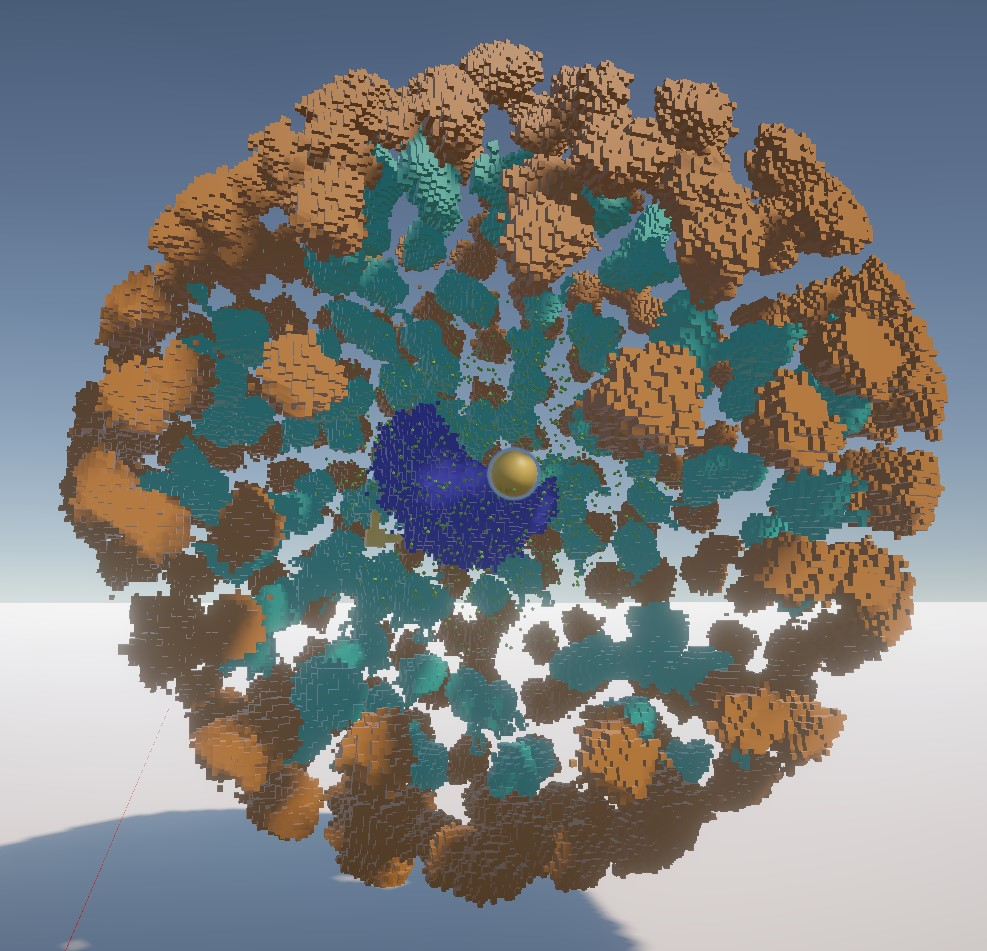
\includegraphics[width=0.7\linewidth]{fig/Images/largeDataset}
	\caption[]{Last time step of a data set with 448 parts.}
	\label{fig:largeDataset}
\end{figure}
A performance analysis was conducted to test the scalability of the methods. The program structure used runs at an average of 101 frames per second on datasets with 448 individual cells at thirty time steps on a computer with an NVIDIA GeForce GTX 970 and an Intel(R) Core(TM) i7-5820K. This is also the largest data set tested and can be seen in figure \ref{fig:largeDataset}. In this dataset, showing the last timestep over 9.5 million tris are active and need to be rendered. During the last time step the cell complex is at its largest state and the most individual cells are displayed. The render time here in the editor is 13.4 milliseconds on average, so an average of 74.4 frames per second. The CPU is the limiting factor here, since there are over 3400 draw calls which increases the render time for such a large number of cells.
The complete results can be seen in figure \ref{tab:performance}. These have been recorded on a standalone process using the point explosion. 
It can therefore be seen that the frames per second decrease with a higher number of parts, but the memory utilization increases primarily with the number of time steps. This was to be expected due to the program structure used. 
The performance is therefore sufficient for the required visualization and better than expected, but could still be significantly optimized. First of all, a reduction in the number of draw calls should be attempted, which should greatly improve the performance for time steps with many parts. The choice of Unity's Universal Rendering Pipeline has proven to be useful. Furthermore, the number of vertices could be reduced substantially, as currently each voxel is represented as a cube with six sides, i.e. 12 tris.
This could be limited to only the surface structure of the cells when importing the dataset, thus massively reducing the tris count. Furthermore, running the program within the editor greatly affects performance. Here, a GUI must also be rendered and additional debug information is displayed.If the program is exported as executable, this also increases the performance, but some options are only usable via the UI panel of the editor. 
Since the data set is imported and completely computed at the program start, the initial load-up time becomes longer with increasing data set sizes. Also each time step remains loaded permanently in the memory, which could also become a bottleneck. This could be prevented if the time steps were loaded dynamically, but could also lead to problems, since the meshes of the cells would have to be calculated at runtime. The implementation of the line visualization is also in need of improvement. This currently adds a new object per line and therefore quickly reduces the performance. Since this visualization, however, did not prove to be useful, it was not addressed. This could be rectified by combining the individual lines to a single mesh and object or by drawing the lines on the GPU. The program structure used has proven to be very robust, which not only delivers performant results, but is also easily expandable.


\begin{table}[h]
	\centering
	\caption{Performance analysis results of different data sets using the point explosion. $\delta$ is the maximum number of simultaneously active cells.}
	\label{tab:performance}
	\renewcommand{\arraystretch}{1.3}
	\begin{tabular}{@{}lllll@{}}
		\toprule
		Dataset name          &    $\delta$     & average FPS     & number of time steps  & memory allocated (MB)            \\ \midrule
		Example-CellSorting-3D     & 60  & 170 & 10 &  204       \\ 
		VirtualEmbryo\_1 &  189  & 160  &  10 & 272  \\ 
		VirtualEmbryo\_2 & 392  &  145  &  12 & 465   \\
		VirtualEmbryo\_3 & 419 &  130 & 14 & 732  \\
		VirtualEmbryo\_4 & 448 & 101 & 30 & 1228  \\\bottomrule
	\end{tabular}
\end{table}
